%!TEX TS-program = xelatex
%!TEX encoding = UTF-8 Unicode
\documentclass[12pt,a4paper]{article}
\usepackage{geometry} % 設定邊界
\geometry{
  top=1in,
  inner=1in,
  outer=1in,
  bottom=1in,
  headheight=3ex,
  headsep=2ex
}
\usepackage{fontspec} % 允許設定字體
\usepackage{xeCJK} % 分開設置中英文字型
\usepackage{url} % 使用url
\usepackage[colorlinks,
            linkcolor= black]{hyperref}
\setCJKmainfont{LiHei Pro} % 設定中文字型
\setmainfont{Georgia} % 設定英文字型
\setromanfont{Georgia} % 字型
\setmonofont{Courier New}
\linespread{1.2}\selectfont % 行距
\XeTeXlinebreaklocale "zh" % 針對中文自動換行
\XeTeXlinebreakskip = 0pt plus 1pt % 字與字之間加入0pt至1pt的間距,確保左右對整齊
\parindent 0em % 段落縮進
\setlength{\parskip}{20pt} % 段落之間的距離

\title{\huge 物聯網應用與資料分析 Assignment1 - MySQL+Arduino+Java
Web+Highchart} % 設置標題,使用巨大字體
\author{姓名:吳嘉偉\quad 學號:5105056013\quad 日期:2018/3/17} % 設置作者
\date{} % 設置日期
\usepackage{titling}
\setlength{\droptitle}{-8em} % 將標題移動至頁面的上面
\usepackage{listings}

% 設置演算法的灰色底
\usepackage{algorithmic}
\usepackage{color}
\definecolor{algorbgm}{gray}{0.85}
\newcommand{\grayblock}[1]{
\colorbox{algorbgm}{\centering
\begin{minipage}{0.8\textwidth} ~\\[-15pt]#1~\\[-25pt] \end{minipage}}}
% example
%\begin{algorithmic}
%\IF{somebody open the door 1}
%\STATE he gets an apple
%\STATE he gets an key
%\ELSIF{somebody open the door 2}
%\STATE he gets nothing
%\ENDIF
%\end{algorithmic}

% 設置灰底
\usepackage{color}
\usepackage{framed}
\definecolor{shadecolor}{gray}{0.85}
% example
%\begin{shaded}
%java -jar test.jar	
%\end{shaded}

\begin{document}

\clearpage

\maketitle % 顯示標題

\section{目標}
{
\fontsize{14pt}{10pt} % 字型大小14pt,字行間距20pt
\selectfont % 生效
利用Arduino輸出數值,透過Java讀值後寫入MySQL,最後再透過PHP跟MySQL取得數值並畫出曲線產生在網頁上。
\begin{figure}[ht]
\centering
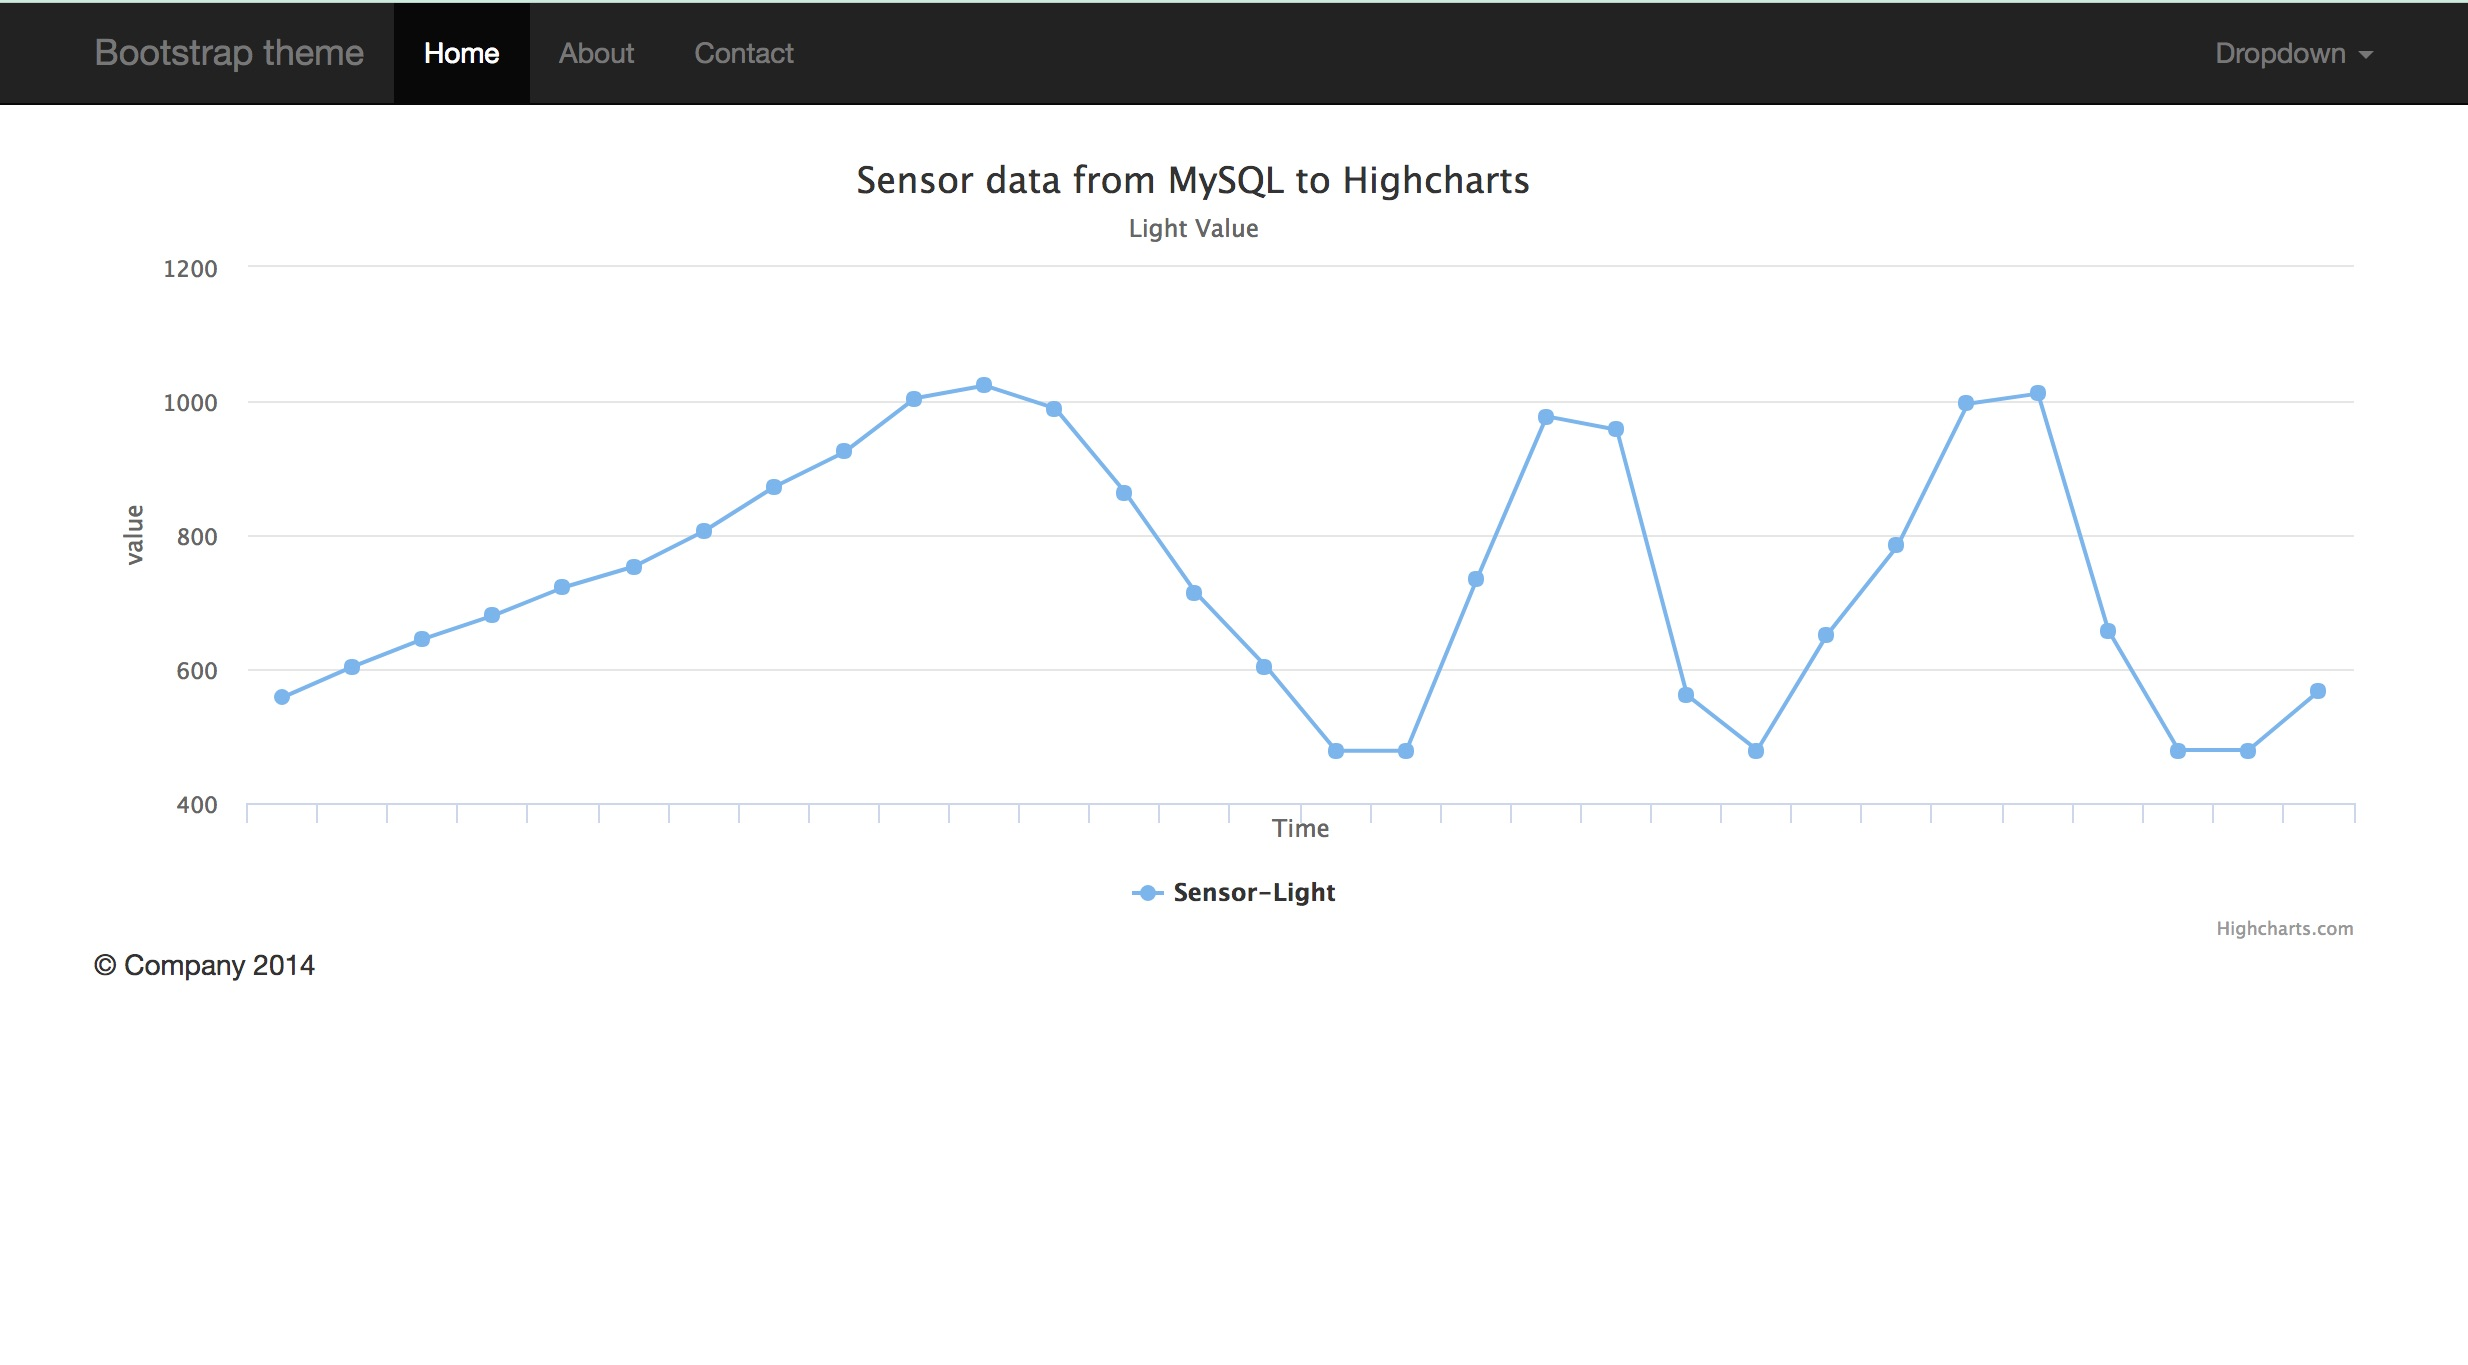
\includegraphics[width=1.0\textwidth]{image/highcharts.jpg}
\end{figure}
}

\newpage % 新一頁
\section{Arduino}
{
\subsection{接腳圖}
利用Arduino、麵包板、可變電阻、10KΩ電阻
\begin{figure}[ht]
\centering
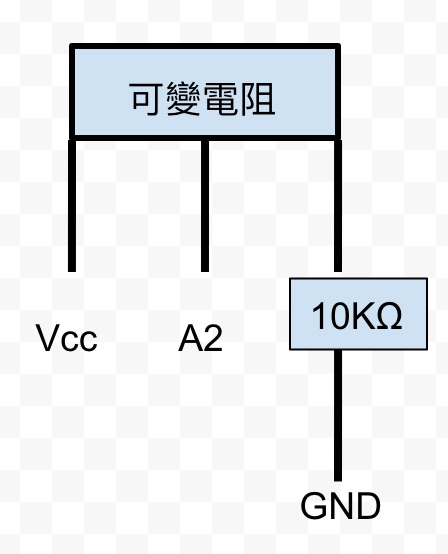
\includegraphics[width=.6\textwidth]{image/接腳示意圖.jpg}
\centering
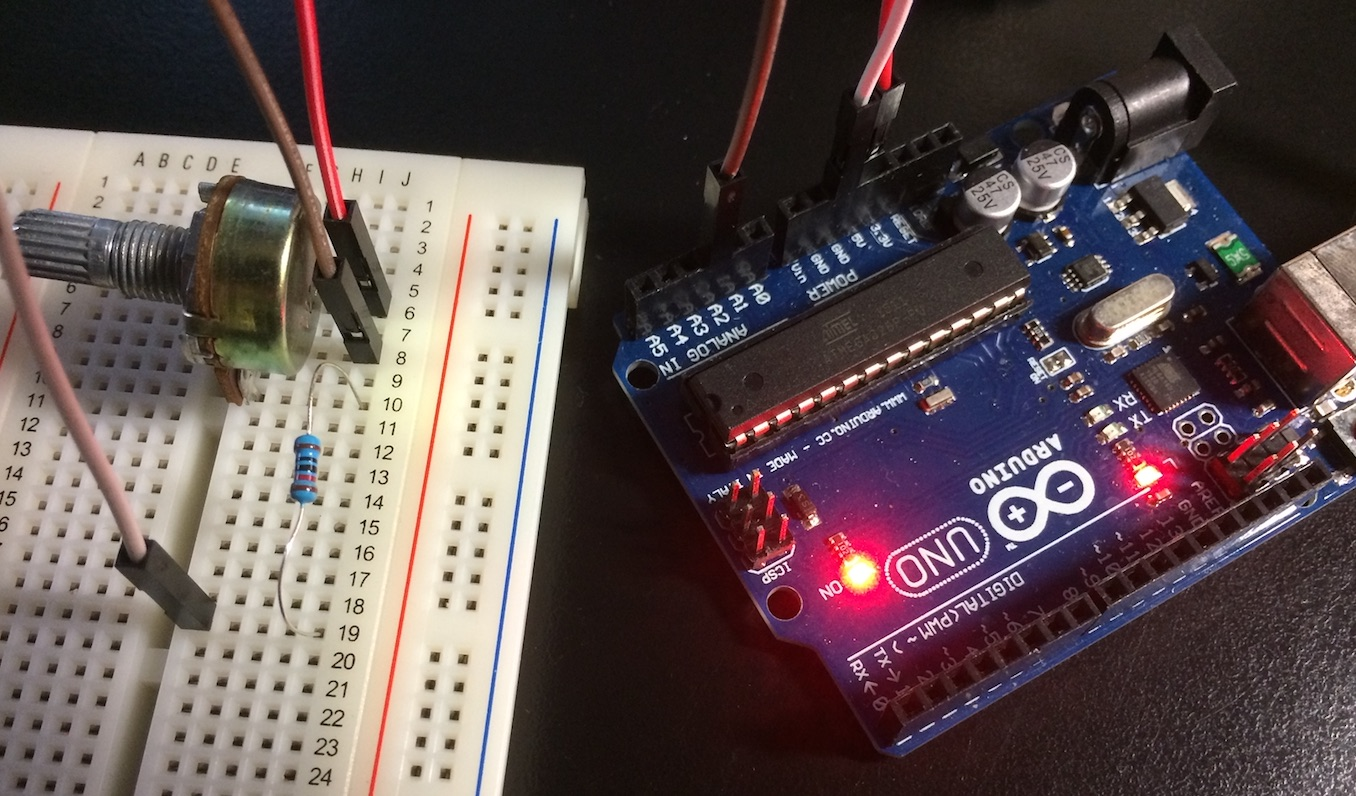
\includegraphics[width=.6\textwidth]{image/接腳圖.jpg}
\end{figure}

\subsection{取得Arduino輸出的數值}

程式碼:
\begin{shaded}
\begin{lstlisting}[language=Arduino]
int pin = A2;

void setup()
{
  Serial.begin(9600);
}

void loop()
{
  int value = analogRead(pin);
  Serial.println(value);
  delay(1000);
}
\end{lstlisting}
\end{shaded}

輸出情況:
\begin{figure}[ht]
\centering
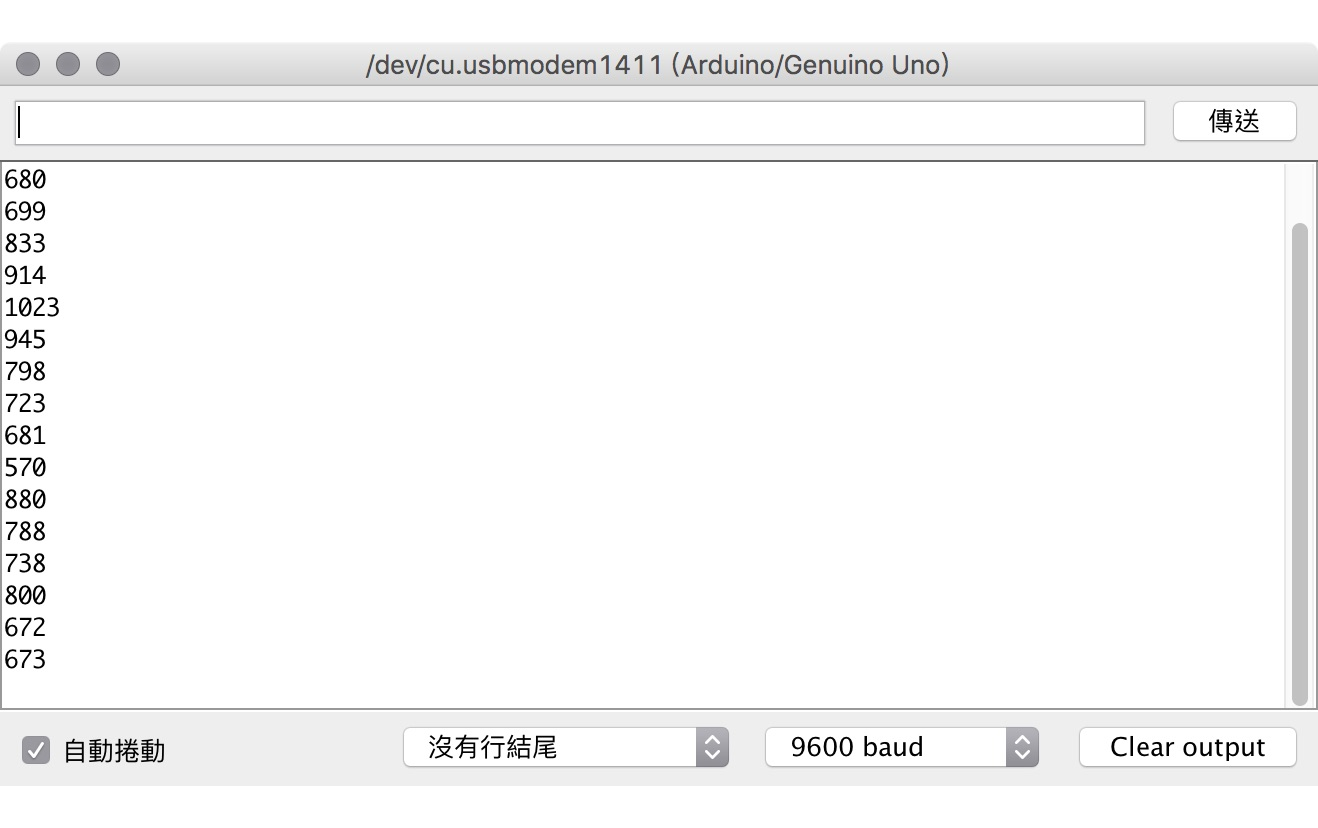
\includegraphics[width=1.0\textwidth]{image/arduino_output.jpg}
\end{figure}

\subsection{利用Java讀取Arduino數值}

此次使用的平台是MacOS,所以port ID是"/dev/cu.usbmodem1411",另外,要知道如何在MacOS上實作可以參考我寫的另外一篇
\href{https://medium.com/@willywu/rxtx-serial-ports-on-macos-8e99b3c7a001}{RXTX, Serial ports on macOS}

擷取部分重要程式碼:
\begin{shaded}
\begin{lstlisting}[language=Java]
//掃過所有的port
while (portEnum.hasMoreElements()) {
  //定義currPortId
  CommPortIdentifier currPortId = 
	  (CommPortIdentifier)portEnum.nextElement();
  //設定arduino serial port
  if (currPortId.getName().equals("/dev/cu.usbmodem1411")) {
	  portId = currPortId;
	  break;
  }
}
\end{lstlisting}
\end{shaded}

數值顯示在Console:
\begin{figure}[ht]
\centering
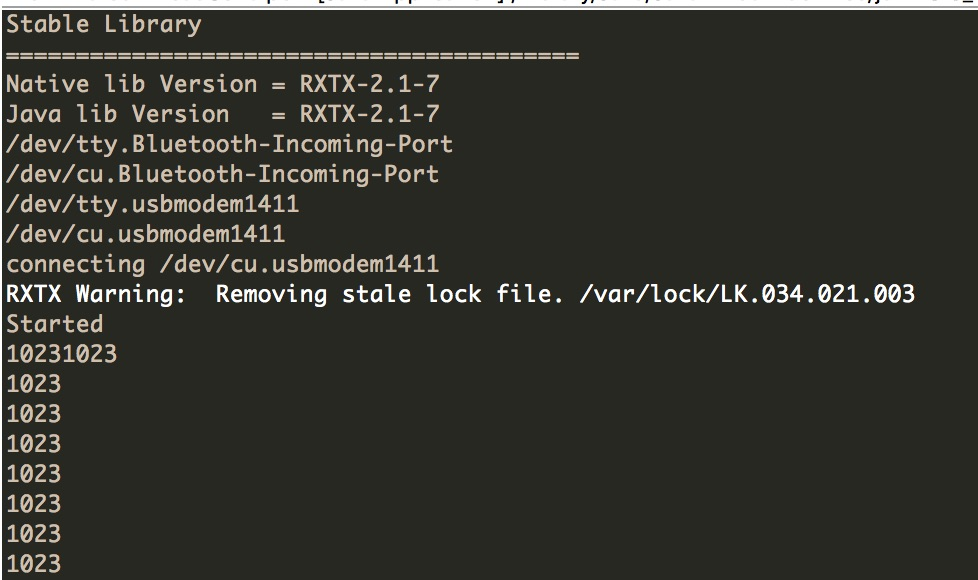
\includegraphics[width=1.0\textwidth]{image/console.jpg}
\end{figure}
}

\newpage
\section{MySQL}
{
\subsection{建立資料庫資料}
利用XAMPP,用網頁連接到http://localhost/phpmyadmin
並建立此次作業需要的資料庫

\begin{figure}[ht]
\centering
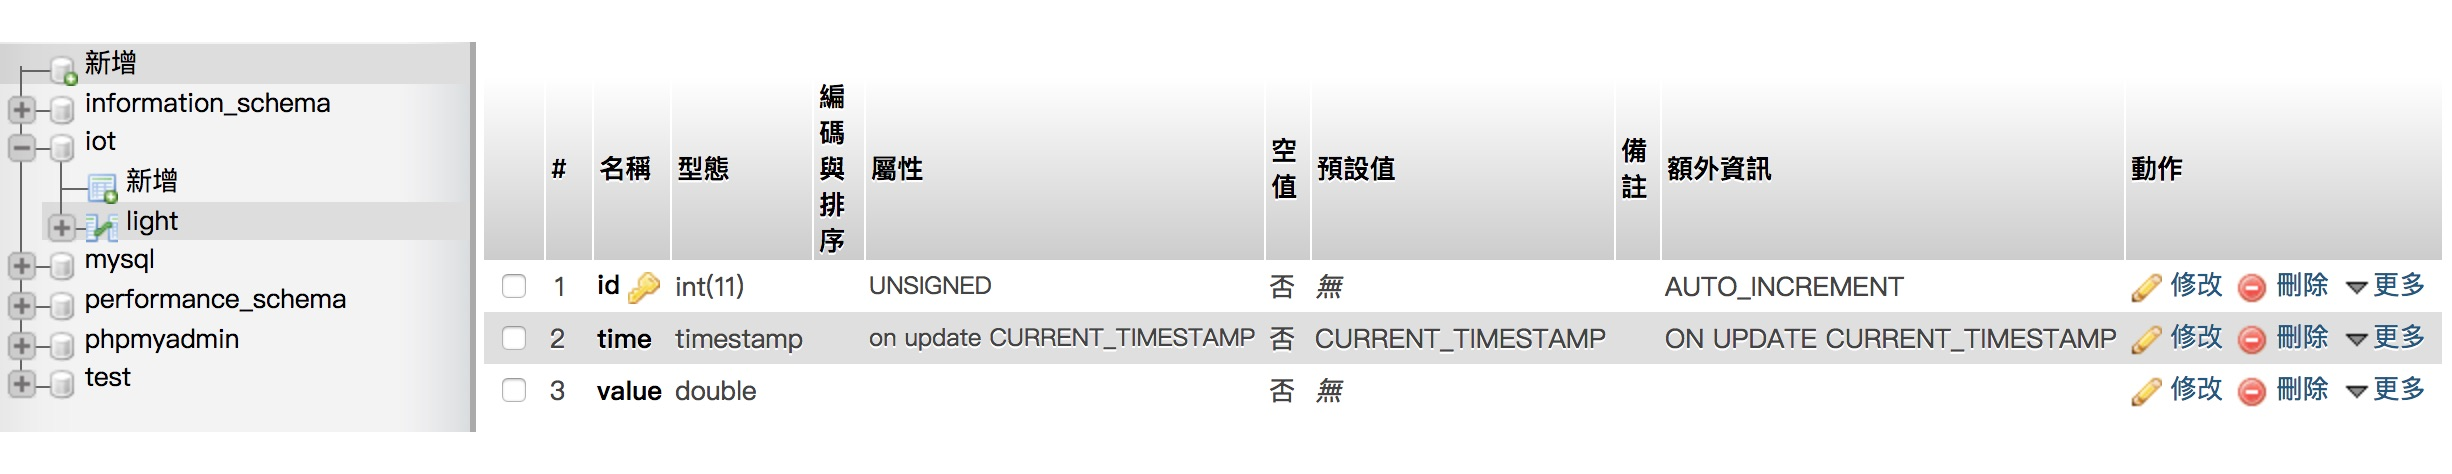
\includegraphics[width=1.0\textwidth]{image/table.jpg}
\end{figure}

\subsection{Java寫值進MySQL}
在Java上設定資料庫的資料
\begin{shaded}
\begin{lstlisting}[language=Java]
//設定server IP,帳號,密碼

//設定JDBC driver  
static final String JDBC_DRIVER = "com.mysql.jdbc.Driver";
//server IP後街資料庫名稱
static final String DB_URL = "jdbc:mysql://192.168.1.111/iot";
static final String USER = "iot";
static final String PASS = "iot";
\end{lstlisting}
\end{shaded}

\newpage
Console:
\begin{figure}[ht]
\centering
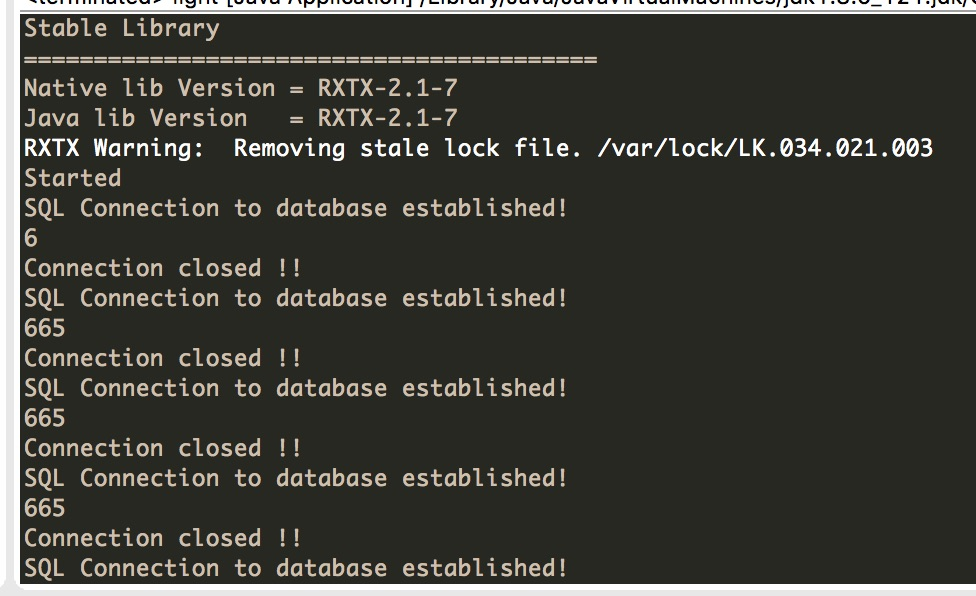
\includegraphics[width=1.0\textwidth]{image/datatomysql.jpg}
\end{figure}

\subsection{Java連接MySQL讀值}
透過Java連接MySQL,並取出剛剛寫入的數值
\begin{shaded}
\begin{lstlisting}[language=Java]
//建立一個物件傳送SQL statement到database
statement = (Statement) connection.createStatement();
String sql= "SELECT * FROM light";
//執行sql語法,回傳語法結果
ResultSet rs = statement.executeQuery(sql);
	while(rs.next()){
	    //檢索每行的欄位
	    int id  = rs.getInt("id");
	    int value = rs.getInt("value");
	    //將value print出來
	    System.out.print("Id: " + id);
	    System.out.println(", Value: " + value);
	 }
\end{lstlisting}
\end{shaded}

\newpage
Console:
\begin{figure}[ht]
\centering
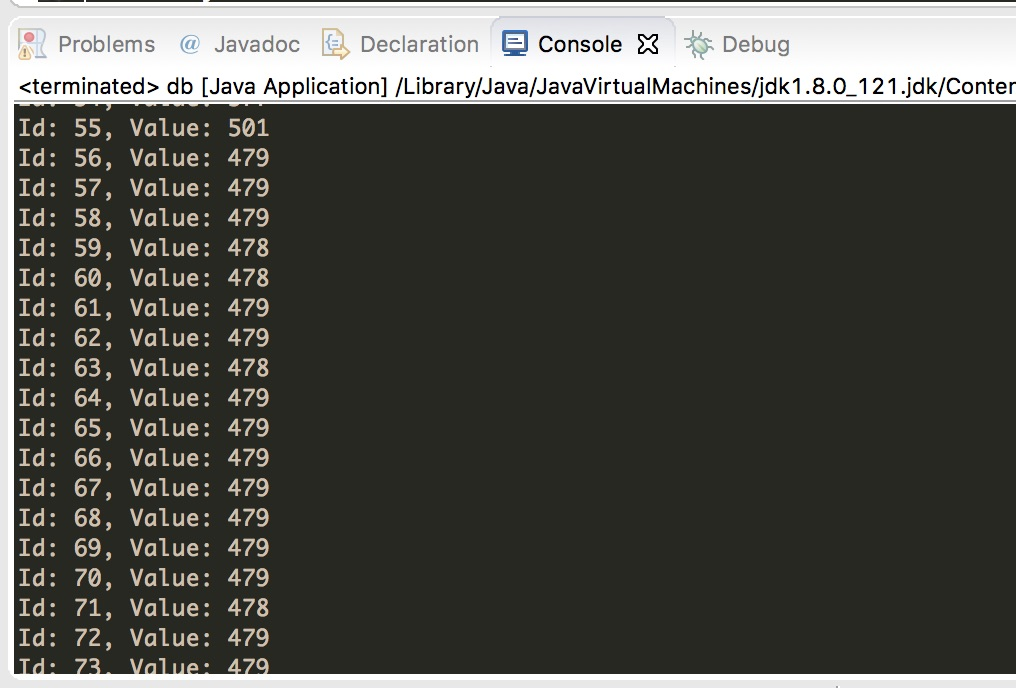
\includegraphics[width=1.0\textwidth]{image/mysqldata.jpg}
\end{figure}

\subsection{產生light.jar檔}
把Java寫數值入MySQL的class匯出(此處是把老師提供的datatomysql這份專案匯出),產生light.jar檔案。
並從Terminal執行jar檔,並持續的寫值進入MySQL中。

開啟Terminal,並輸入以下指令
\begin{shaded}
\begin{lstlisting}[language=Java]
java -jar light.jar
\end{lstlisting}
\end{shaded}

\newpage
下圖可以看到,Terminal上顯示light.jar一直在把數值寫入MySQL 
\begin{figure}[ht]
\centering
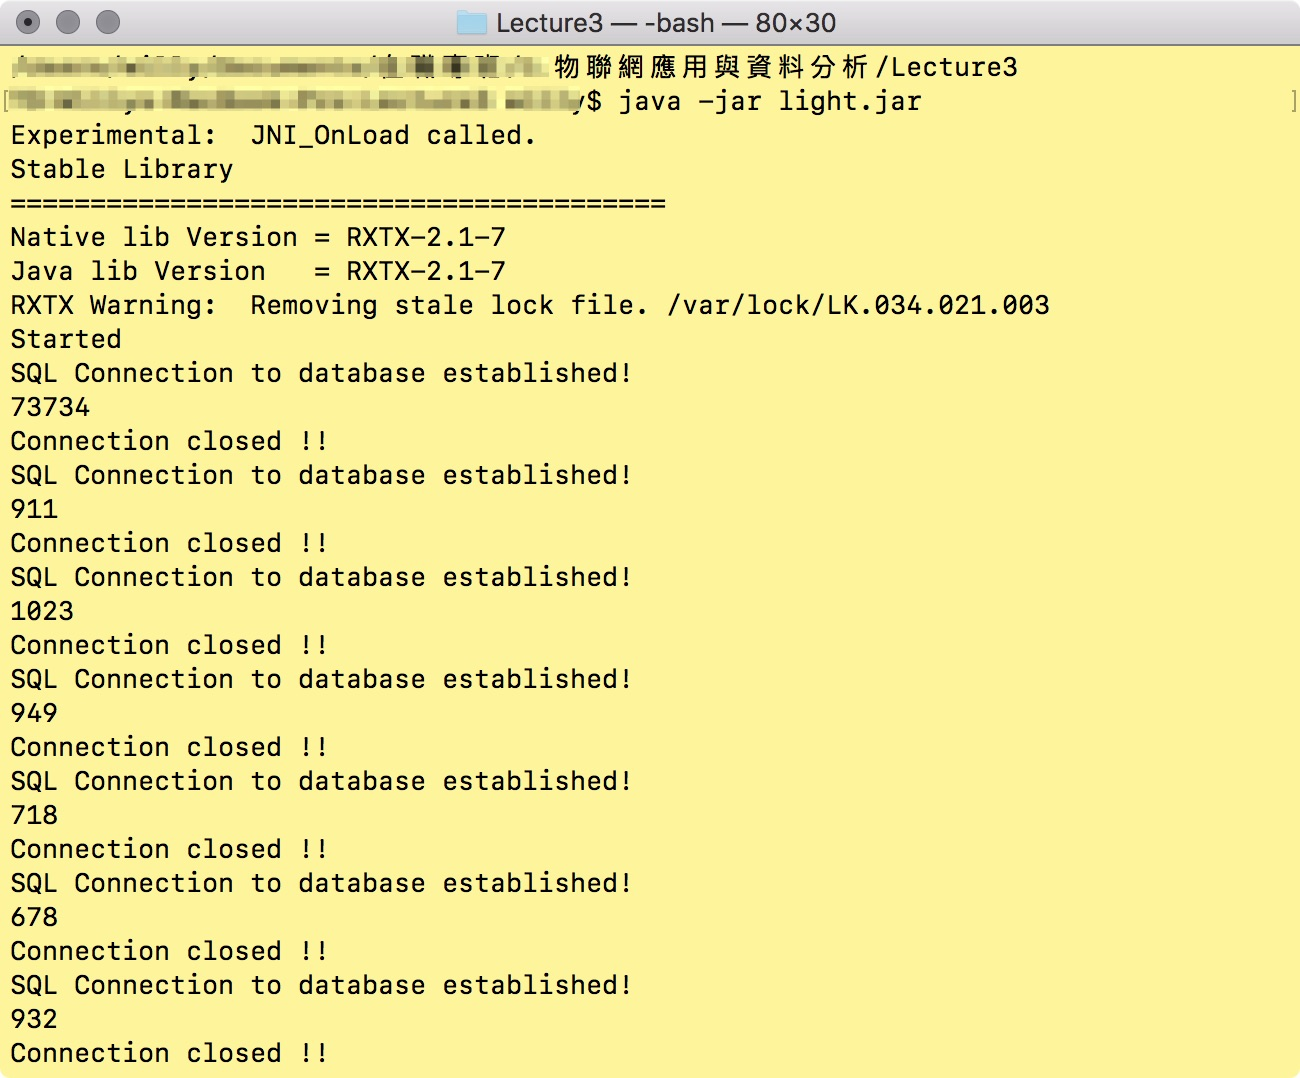
\includegraphics[width=1.0\textwidth]{image/consoletomysql.jpg}
\end{figure}
}

\newpage
\section{Web}
{
\subsection{PHP}
填入MySQL的一些重要資訊。
需注意原本提供的程式碼是使用新版已經被deprecated的function
所以執行上會有錯誤,基本上是把mysql改成mysqli,並調整帶入的參數即可
\begin{shaded}
\begin{lstlisting}[language=Java]
<?php
  //user information
  $host = "192.168.1.111";
  $user = "iot";
  $pass = "iot";

  //database information
  $databaseName = "iot";
  $tableName = "light";

  //Connect to mysql database
  $con = mysqli_connect($host,$user,$pass);
  $dbs = mysqli_select_db($con, $databaseName);


  //Query database for data
  $result = mysqli_query($con, "SELECT * FROM $tableName");

  //store matrix
  $i=0;
  while ($row = mysqli_fetch_array($result)){
    $employee[$i]=$row;
    $i++;
  }

  //echo result as json 
  echo json_encode($employee);
?>
\end{lstlisting}
\end{shaded}

\newpage
\subsection{High Chart}
畫曲線圖的部分需要注意資料庫比數,因為程式上需要大於30筆,才會顯示
所以當你一開始資料筆數不夠的話會造成曲線圖出不來
\begin{figure}[ht]
\centering
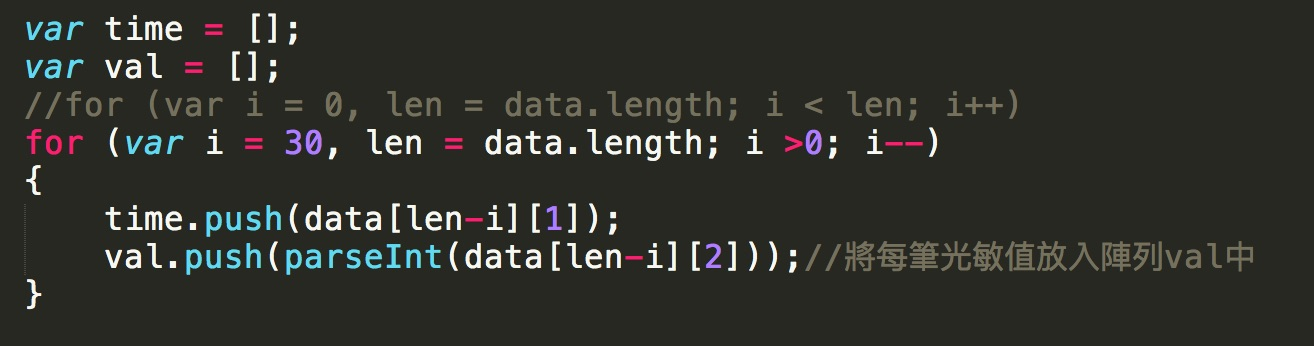
\includegraphics[width=1.0\textwidth]{image/highchart.jpg}
\end{figure}

\subsection{執行結果}
最後都完成後,從網頁進入http://localhost/iot/highchart.html就可以看到下圖
這時候只要轉動可變電阻,即可看到曲線變化
\begin{figure}[ht]
\centering
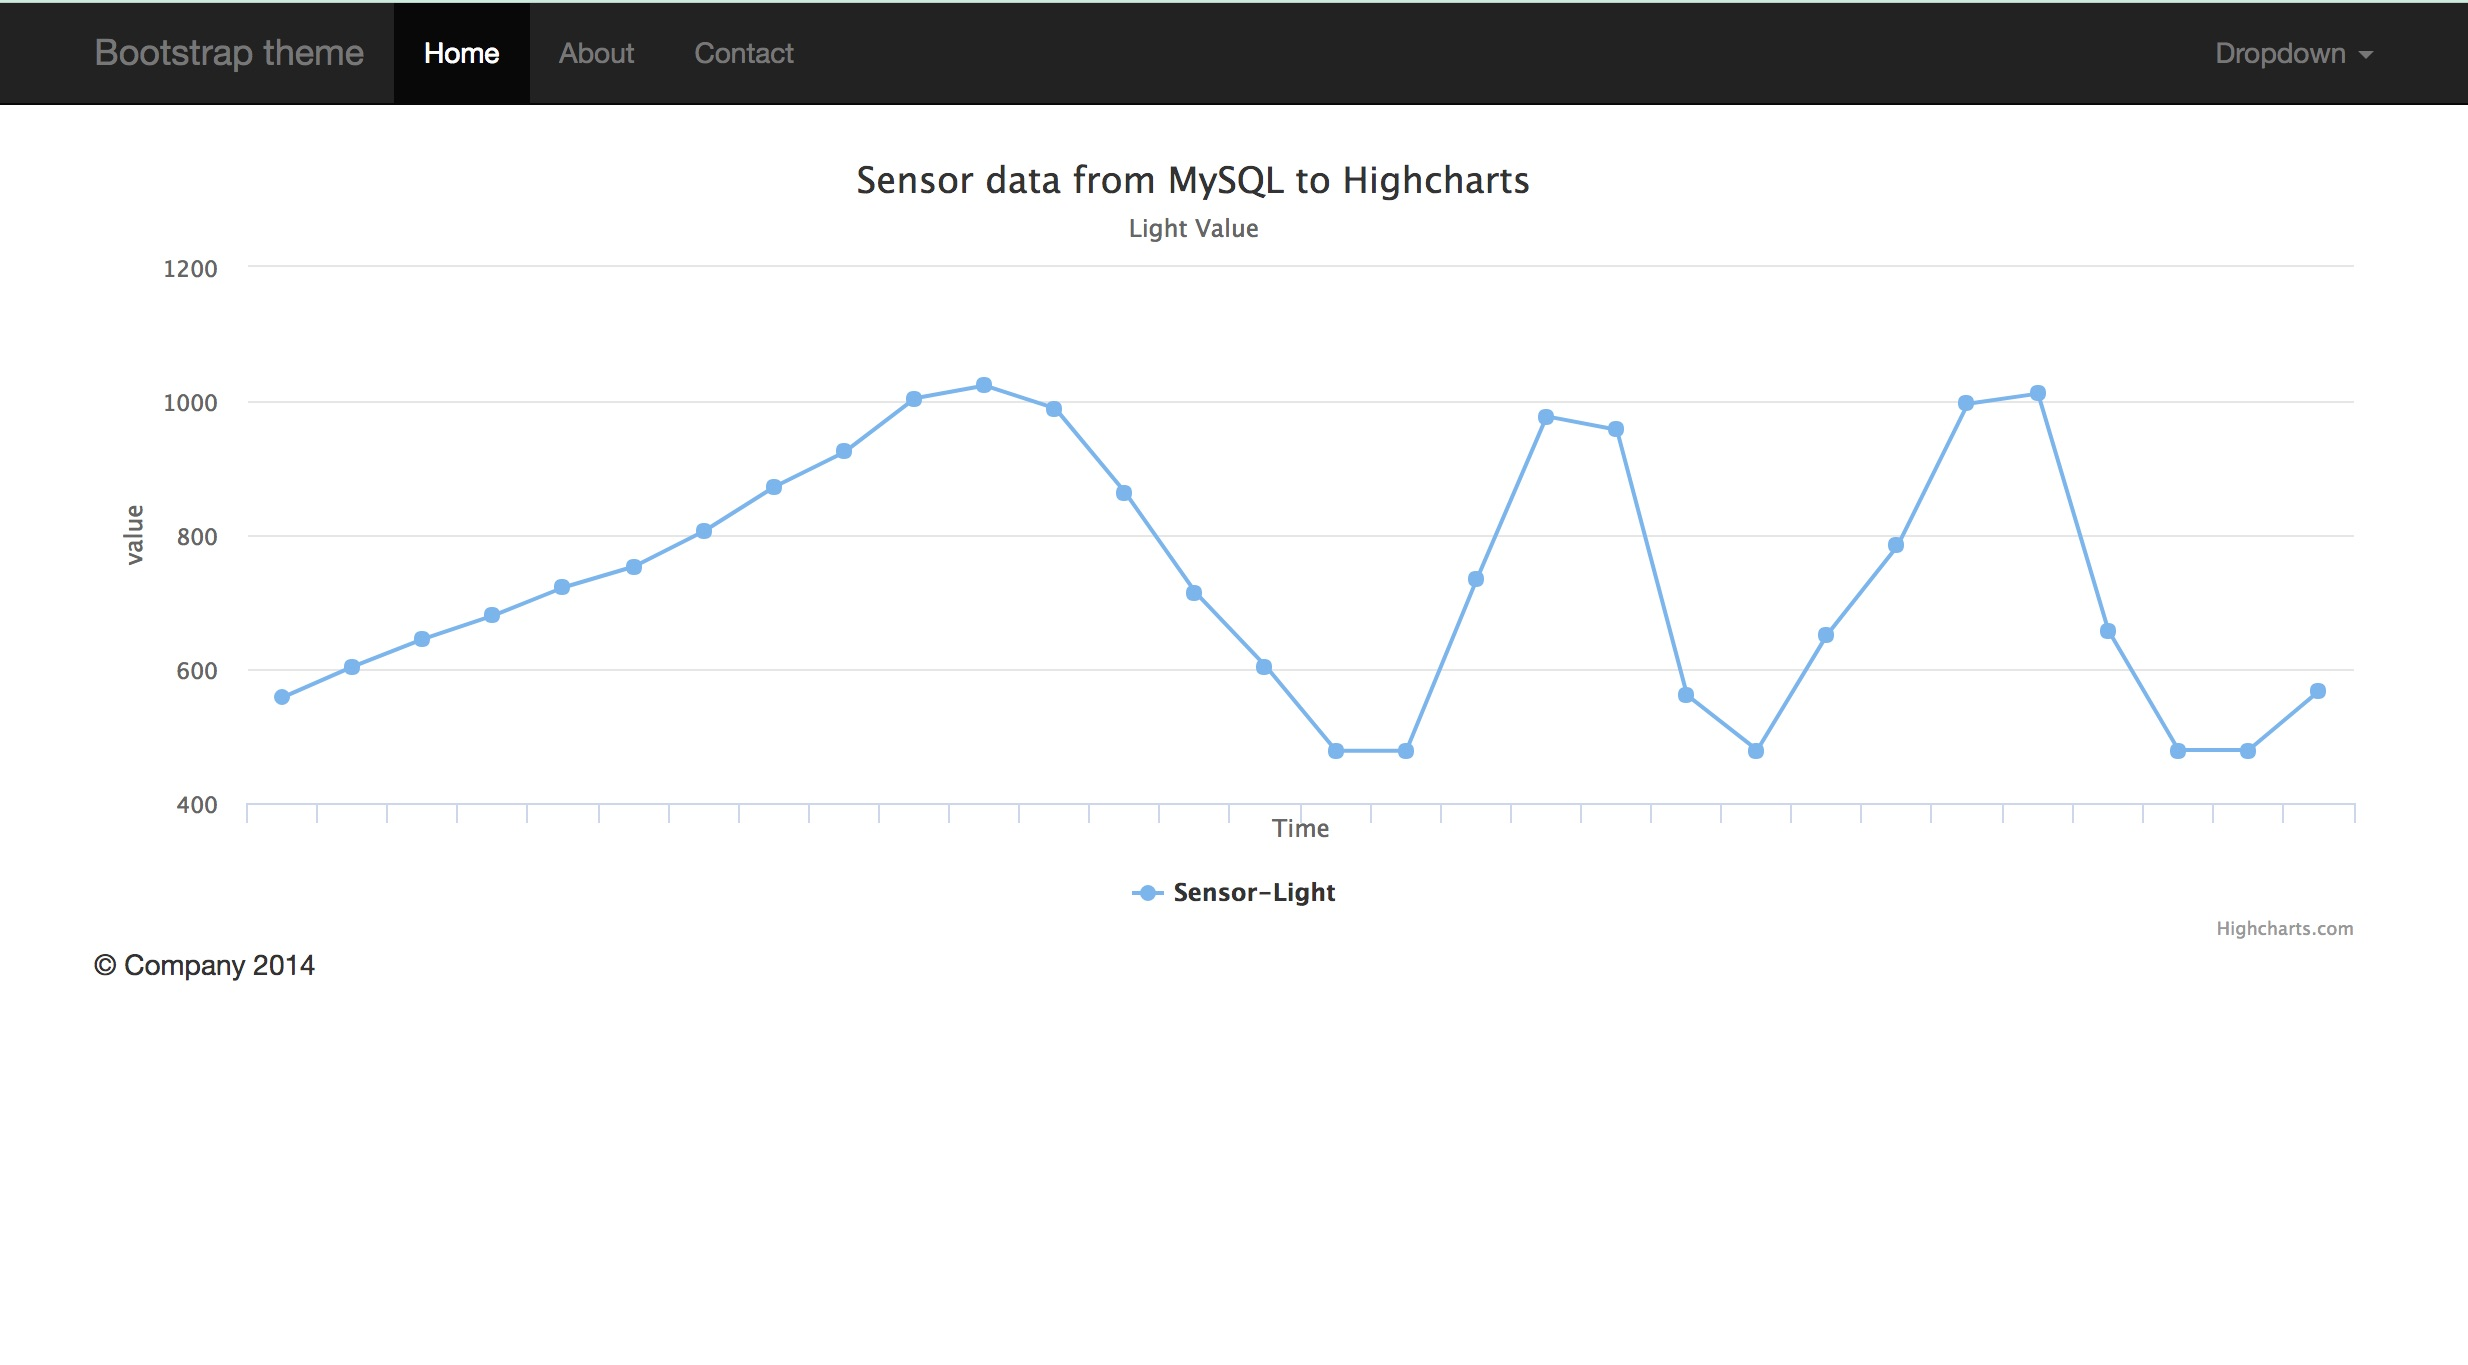
\includegraphics[width=1.0\textwidth]{image/highcharts.jpg}
\end{figure}
}

\end{document}